\begin{vplace} % vertically centered environment
\thispagestyle{empty}


\includegraphics[height=1.9cm]{images/UHH-Logo_2010_Farbe_CMYK}%
\hfill%

\includegraphics[height=3.1cm]{images/wortmarken}

\large
\centering
\newlength{\TitlePageSpacing}
\addtolength{\TitlePageSpacing}{.8cm}

\vspace{2\TitlePageSpacing}

\scshape
\textbf{Physikalisches Praktikum für Fortgeschrittene}\par\bigskip
 
\HUGE\normalfont
\textbf{\ExperimentID{}. \ExperimentTitle}\par

\vspace{.8\TitlePageSpacing}

\scshape

\large
\textbf{Versuchsbeschreibung} \\
Stand: \today{}\par\bigskip

\vspace{\TitlePageSpacing}
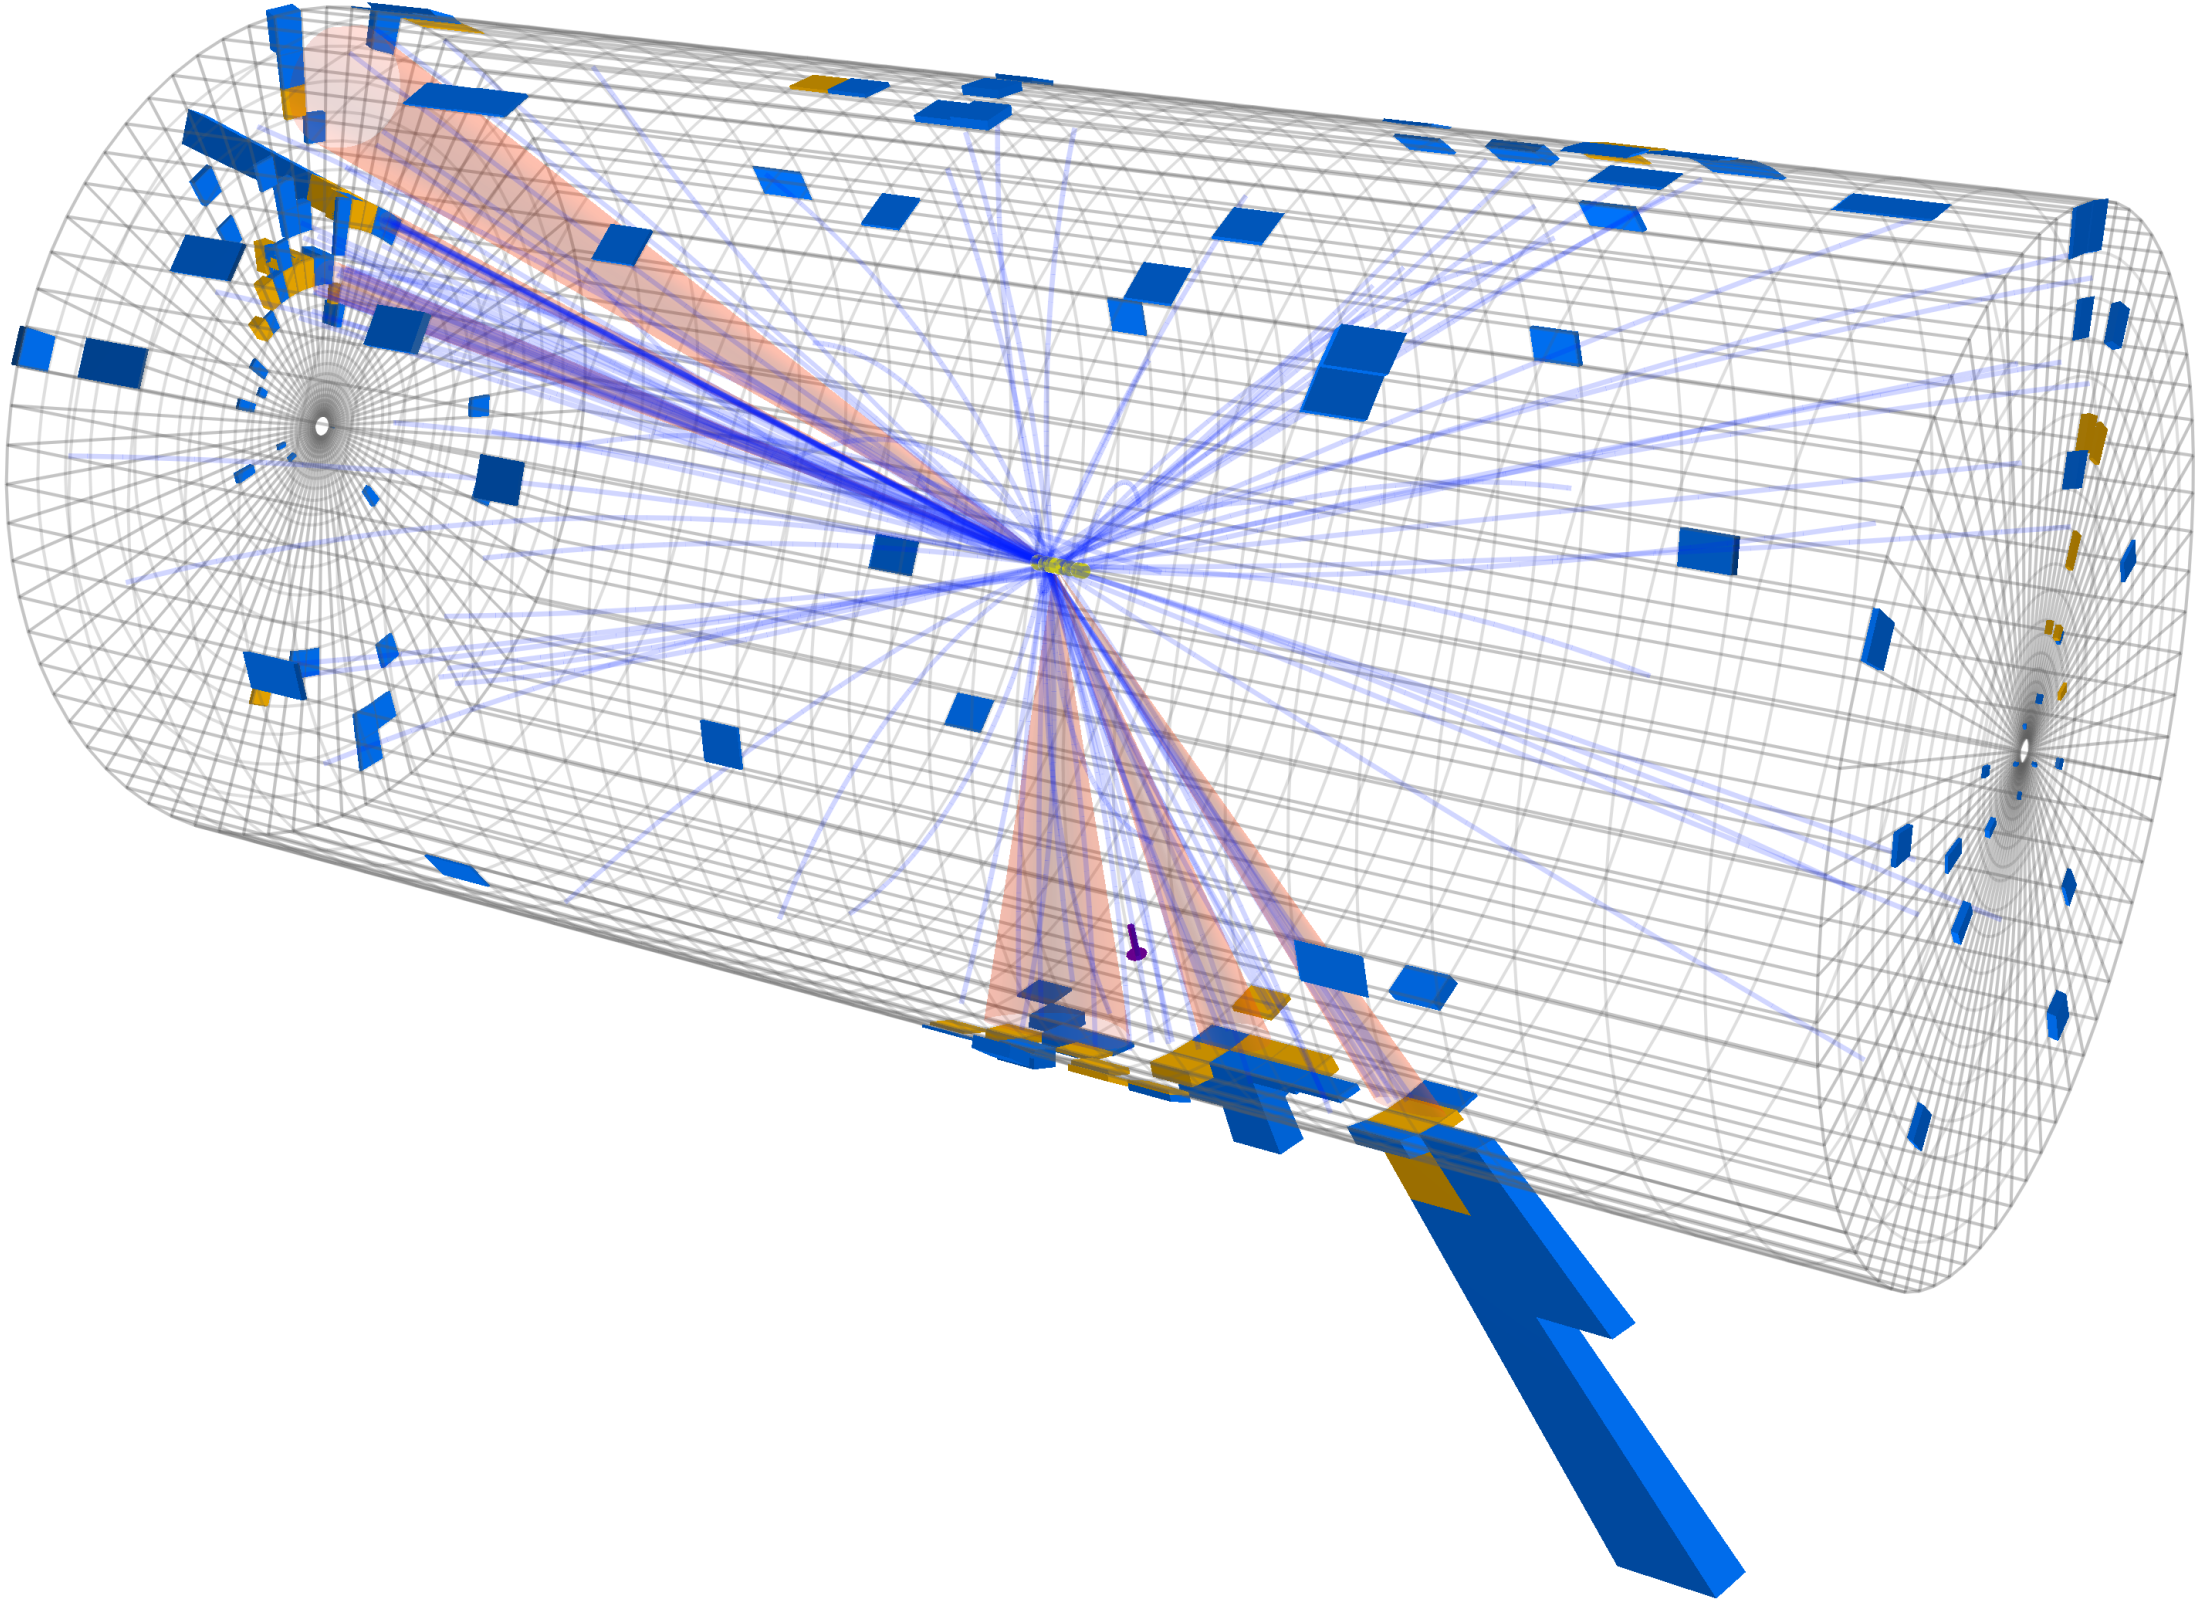
\includegraphics[height=6cm]{images/eventdisplay}
\vspace{\TitlePageSpacing}

\scshape

\textbf{Institut für Experimentalphysik} \\
Arbeitsgruppe Prof. Dr. Johannes Haller \\
Teilchenphysik \& Detektor-Entwicklung\par\bigskip

\textbf{Betreuer:} \\
Alexander Fröhlich \\
Christopher Matthies\par\bigskip

Basierend auf früheren Versionen von \\
A.~Reimers, J.~Multhaup und M.~Stöver

\end{vplace}
